\section{Método}

Se propone utilizar equivalencias entre tipos de datos de FHIR y clases del modelo de referencia de openEHR para creación de arquetipos de openEHR. Éstos tendrán misma estructura y semántica que los recursos definidos en FHIR, permitiendo un modelado común de información entre sistemas que implementan FHIR y openEHR.

Una equivalencia existe si el dominio de valores de un tipo de dato de FHIR puede ser almacenado dentro de uno de los atributos de una de las clases del modelo de referencia de openEHR.

Una vez encontradas las equivalencias, se crearán los arquetipos en un proceso automatizado de 3 etapas: etapa de abstracción, etapa de sustitución y etapa de definición (Figura \ref{fig:solution}).

\begin{figure}
  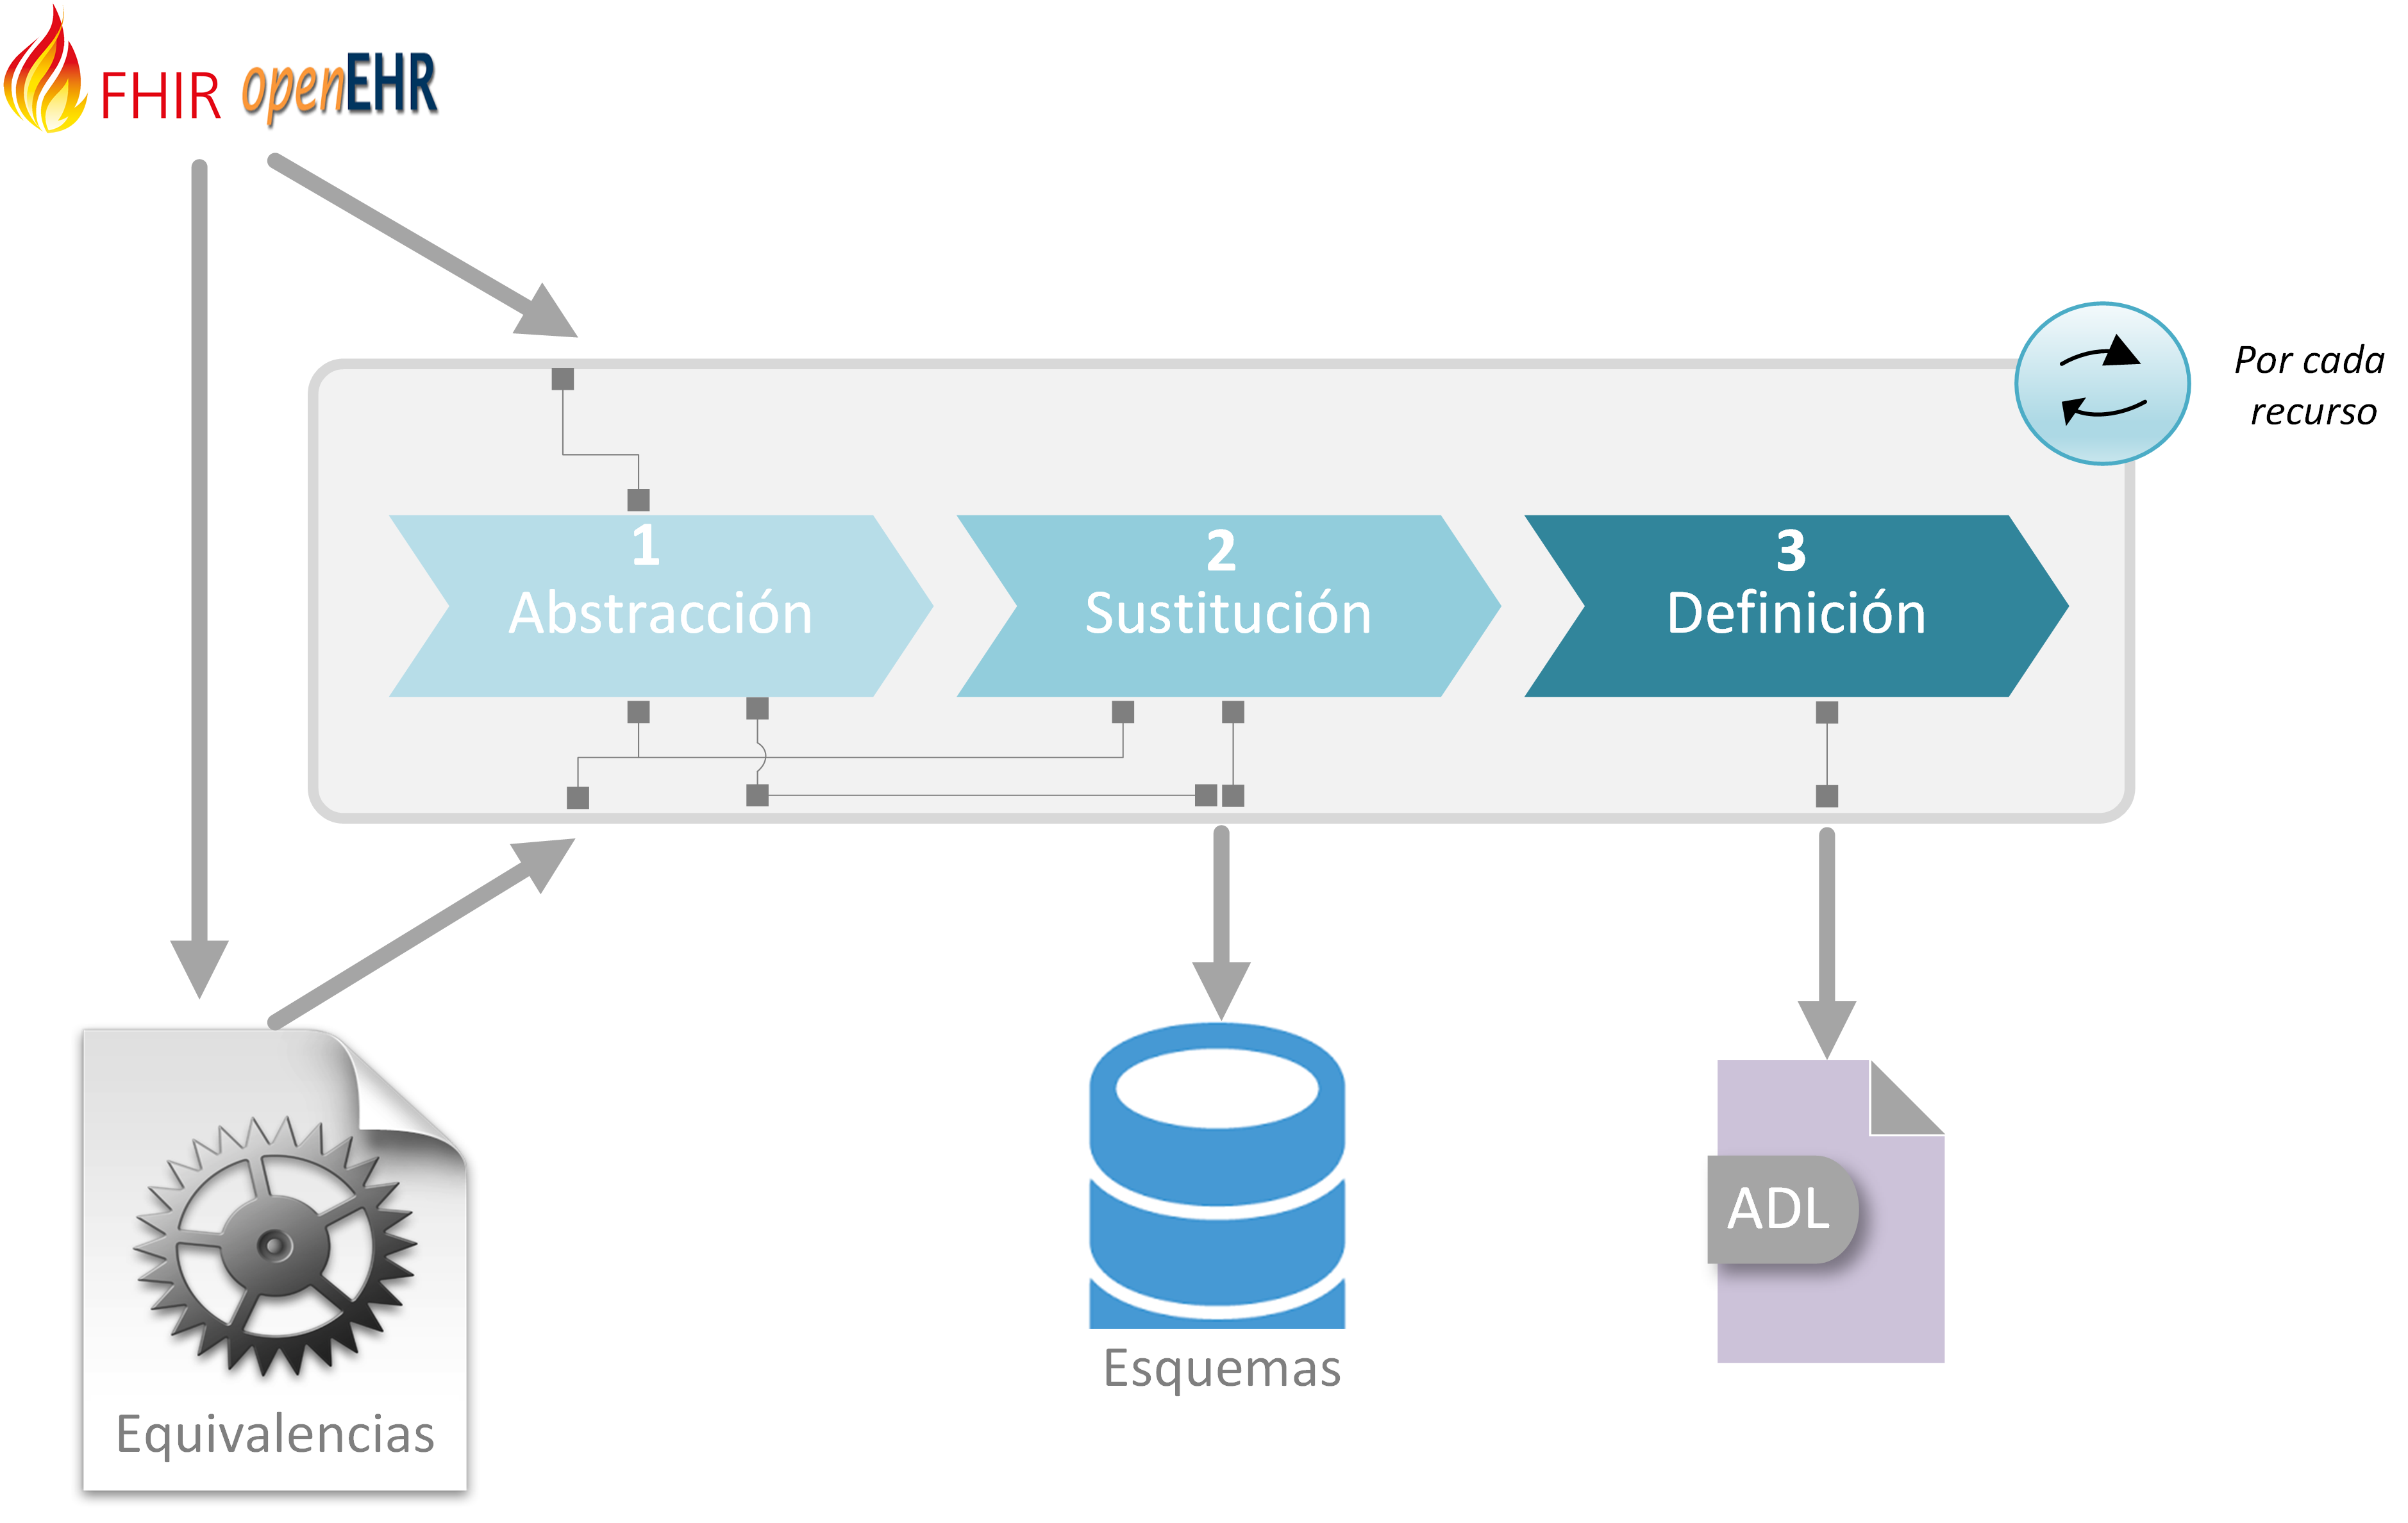
\includegraphics[scale=0.5]{./images/solution}
  \caption{Proceso automatizado}
  \label{fig:solution}
\end{figure}

En las etapas de abstracción y sustitución, se definirán recursos de FHIR dentro de un sistema de tipos de FHIR y openEHR respectivamente, el sistema de tipos será similar al propuesto en \cite{Maldonado09}. Los esquemas, salidas de estas etapas, serán conjuntos de tipos que modelan recursos de FHIR.

En la etapa de definición se transformarán las representaciones de recursos FHIR en sistema de tipos a la sintaxis de arquetipo, la sintaxis a usarse es ADL. La salida de esta etapa son los arquetipos creados.
